% \documentclass{report}
% 
% \usepackage{fancyhdr}
\usepackage{fourier-orns}
\usepackage{hyperref}%% To refrence links / jumps
\usepackage{chngcntr} %% For some extra counters numberings
\usepackage[a4paper, right = 0.5in, left = 0.5in,top = 1in , bottom = 1in]{geometry}
\usepackage{etoolbox} %% Provides like a language for advanced customization
\usepackage{datetime} %% For dates of course
\usepackage{lastpage} %% provides pages numbers
\usepackage[sc]{titlesec} %% modify titles
\usepackage{enumerate}
\usepackage{cancel}
\usepackage{tikzsymbols}
\usepackage[dvipsnames]{xcolor}
\usepackage{import}
\usepackage{pdfpages} %% include other pdfs
\usepackage{transparent} %% Transparency
\usepackage{xcolor}  %% Colors
\usepackage[many]{tcolorbox}
\usepackage[framemethod=TikZ]{mdframed}
\usepackage{amsmath,amsfonts,amsthm,amssymb,mathtools}
\usepackage{tikz}
\usepackage{bookmark}
\usepackage{graphicx}
\usepackage{mathpazo}

\usepackage{fontawesome5}

\linespread{1.5}


\titleformat{\chapter}[display]   
{\fontfamily{ppl}\selectfont\huge\color{YellowOrange!80!orange}} % Font style and size 
{\raggedleft\color{purple}\fontsize{70}{0pt}\selectfont\thechapter}   
{-1.5cm}    			                          % Space between the chapter number and title
{
	\begin{tikzpicture}[overlay]
		\node[anchor = west,yshift = 0.2cm,xshift = -1cm] {\fontsize{90}{20} $\int_{}^{} $};
		\node[yshift = 4cm, xshift = 17cm]   {\includegraphics[width = 4cm]{preview0}};
	\end{tikzpicture}
\hspace{1cm}\Huge\raggedright\MakeUppercase}

\titleformat{\section}[block]
{
\fontfamily{ppl}\selectfont\huge\color{YellowOrange!80!orange}
}
{
\color{purple}\fontsize{20}{0pt}\selectfont\thesection 
}
{0cm}
{
	\begin{tikzpicture}[overlay]
		\node[anchor = west,yshift = 0.2cm,xshift = -0.4cm, circle = 1pt] {};
	\end{tikzpicture}
}

\titlespacing*{\section}{0pt}{0.7cm}{1.5cm}


\newcommand{\divider}
{
	\begin{center}
	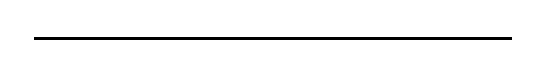
\begin{tikzpicture}
		\draw[thick, black] (0.25*\textwidth, 0) -- (0.75*\textwidth, 0);
		\node[rotate = 360 - 90, xshift = -0.6pt, yshift = 1pt] at (0.25*\textwidth,0){\decotwo};
		\node[rotate = 90, xshift = -0.6pt, yshift = 1pt] at (0.75*\textwidth,0){\decotwo};
	\end{tikzpicture}
	\end{center}
}

\pagestyle{fancy}

\newcommand{\lecday}[1][]
{
    \def\datee{#1}
    \fancyhead[L]{\datee}
}



\newcommand{\signature}
{
	\begin{tikzpicture}[remember picture,overlay]
		\node[fill = YellowOrange!20!white] at ([yshift = 1cm, xshift = -3cm]current page.south east) {\fontsize{10pt}{0pt}{\itshape Kara.$\mathcal{A}$}};
	\end{tikzpicture}
}

\AddToHook{shipout/background}{
  \begin{tikzpicture}[remember picture, overlay]
	  \node[] at ([yshift = 1.5cm,xshift = \textwidth /2 + 0.9cm]current page.south west) {\includegraphics[width = 0.5cm]{preview3}};
	  \node[] at ([yshift = 1.5cm,xshift = - \textwidth /2 - 0.9cm]current page.south east) {\includegraphics[width = 0.5cm]{preview4}};
  \end{tikzpicture}
}



\newtcolorbox[auto counter, number within = section]{remark}[1][]
{
       		title = Remark #1,
		enhanced,
		boxrule = 0pt,
		colback = white,
		breakable,
		arc = 4pt,
		colbacktitle = cyan,
		colback = cyan!5!white,
		segmentation style =
		{
			solid,cyan,thick,
		},
		attach boxed title to top left =
		{
			xshift = 0cm,
		},
		boxed title style =
		{
			boxrule = 0pt,
			sharp corners,
			drop fuzzy shadow = {cyan},
		},
		drop fuzzy shadow = {cyan!80!black},
}

\newtcolorbox[auto counter, number within = section]{theorem}[1][]
{                                      
		title = Theorem \thetcbcounter : #1,
		enhanced, 
		boxrule = 0pt,
		colback = white,
		breakable,
		arc = 4pt,
		colbacktitle = purple,
		colback = purple!5!white,
		segmentation style = 
		{
			solid, purple,thick,
		},
		attach boxed title to top left = 
		{
			xshift = 0cm, 
		},
		boxed title style = 
		{
			boxrule = 0pt,
			sharp corners,
			drop fuzzy shadow = {purple},
		},
		drop fuzzy shadow = {purple!80!black},
}

\newtcolorbox[auto counter, number within = section]{definition}[1][]
{                                      
		title = Definition \thetcbcounter : #1,
		enhanced, 
		boxrule = 0pt,
		colback = white,
		arc = 4pt,
		breakable,
		colbacktitle = YellowOrange!80!black,
		segmentation style = 
		{
			solid, YellowOrange,thick,
		},
		attach boxed title to top left = 
		{
			xshift = 0cm, 
		},
		colback = YellowOrange!5!white,
		boxed title style = 
		{
			boxrule = 0pt,
			sharp corners,
			drop fuzzy shadow = {YellowOrange!80!orange},
		},
		drop fuzzy shadow = {YellowOrange!80!black},
}

\newtcolorbox[auto counter, number within = section]{corollary}[1][]
{                                      
		title = corollary \thetcbcounter : #1,
		enhanced, 
		boxrule = 0pt,
		colback = white,
		arc = 4pt,
		breakable,
		colbacktitle = YellowOrange!80!black,
		segmentation style = 
		{
			solid, YellowOrange,thick,
		},
		attach boxed title to top left = 
		{
			xshift = 0cm, 
		},
		colback = YellowOrange!5!white,
		boxed title style = 
		{
			boxrule = 0pt,
			sharp corners,
			drop fuzzy shadow = {YellowOrange!80!orange},
		},
		drop fuzzy shadow = {YellowOrange!80!black},
}


\newtcolorbox{example}[1][]
{                                      
		title = Example,
		enhanced, 
		boxrule = 0pt,
		colback = white,
		arc = 4pt,
		segmentation style = 
		{
			solid, SpringGreen,thick,
		},
		breakable,
		colback = SpringGreen!5!white,
		colbacktitle = SpringGreen!80!black,
		attach boxed title to top left = 
		{
			xshift = 0cm, 
		},
		boxed title style = 
		{
			boxrule = 0pt,
			sharp corners,
			drop fuzzy shadow = {SpringGreen!80!orange},
		},
		drop fuzzy shadow = {SpringGreen!80!black},
}


\newcommand{\integral}[4]{\int\limits_{#1}^{#2} #4 d#3}
\newcommand{\limit}[3]{\lim\limits_{#1 \rightarrow #2} #3}
\newcommand{\strone}[2]{\left[ \begin{gathered}#1\\ #2\end{gathered} \right] }
\newcommand{\strtwo}[2]{\left\{ \begin{gathered}#1\\ #2\end{gathered} \right\} }
\newcommand{\strthree}[2]{\left\lfloor \begin{gathered}#1\\ #2\end{gathered} \right\rfloor }


\newcommand{\startbf}[1]{\text{\bfseries{#1}}}
\newcommand{\sett}[1]{\left\{ #1 \right\}}
\newcommand{\thesis}[1]{\left( #1 \right)}
\newcommand{\brkt}[1]{\left[ #1 \right]}
\newcommand{\floor}[1]{\left\lfloor #1 \right\rfloor}


\DeclareMathOperator{\img}{im} % Image
\DeclareMathOperator{\Img}{Im} % Image
\DeclareMathOperator{\coker}{coker} % Cokernel
\DeclareMathOperator{\Coker}{Coker} % Cokernel
\DeclareMathOperator{\Ker}{Ker} % Kernel
\DeclareMathOperator{\rank}{rank}
\DeclareMathOperator{\Spec}{Spec} % spectrum
\DeclareMathOperator{\Tr}{Tr} % trace
\DeclareMathOperator{\pr}{pr} % projection
\DeclareMathOperator{\ext}{ext} % extension
\DeclareMathOperator{\pred}{pred} % predecessor
\DeclareMathOperator{\dom}{dom} % domain
\DeclareMathOperator{\ran}{ran} % range
\DeclareMathOperator{\Hom}{Hom} % homomorphism
\DeclareMathOperator{\Mor}{Mor} % morphisms
\DeclareMathOperator{\End}{End} % endomorphism


\newcommand{\lm}{\ensuremath{\lambda}}
\newcommand{\eps}{\ensuremath{\epsilon}}
\newcommand{\veps}{\ensuremath{\varepsilon}}
\newcommand{\al}{\ensuremath{\alpha}}
\newcommand{\bb}{\ensuremath{\beta}}
\newcommand{\cc}{\ensuremath{\gamma}}
\newcommand{\dd}{\ensuremath{\delta}}
\newcommand{\DD}{\ensuremath{\Delta}}
\newcommand{\ff}{\ensuremath{\phi}}
\newcommand{\FF}{\ensuremath{\varphi}}

\newcommand{\RR}{\mathbb{R}}
\newcommand{\RO}{\mathcal{R}}
\newcommand{\EE}{\mathbb{E}}
\newcommand{\CC}{\mathbb{C}}
\newcommand{\RW}{\mathbb{R}^2}
\newcommand{\RT}{\mathbb{R}^3}
\newcommand{\RN}{\mathbb{R}^n}
\newcommand{\DS}{\mathcal{D}}

\newcommand{\KK}{\mathbb{K}}
\newcommand{\KW}{\mathbb{K}^2}
\newcommand{\KT}{\mathbb{K}^3}
\newcommand{\KN}{\mathbb{K}^n}

\newcommand{\NN}{\mathbb{N}}

\newcommand{\PS}{\mathcal{P}}
\newcommand{\AS}{\mathcal{E}}
\newcommand{\FS}{\mathcal{F}}
\newcommand{\LS}{\mathcal{L}}
\newcommand{\MS}{\mathcal{M}}


















\lecday[2025-02-13]

% \begin{document}

\begin{theorem}[]
Let $E$ be a $\KK$-Vector space and let
$N_1$ and $N_2$ be two norms on $E$, then we have
equivalence between : 
\begin{enumerate}[(i)]
\item $N_1$ and $N_2$ are toplogically equivalent
\item $N_1$ and $N_2$ are equivalent 
\end{enumerate}
\end{theorem}
\begin{proof}
we have
\[
\begin{array}{cccc}
      id_{E} : &  \left( E,N_1 \right)  & \longrightarrow & 
      \left( E,N_2 \right)\\

           &  x  & \longmapsto     & x \\ 
\end{array}
\]
is bicontinious, and it's bi-Lipschitz continious. But
since $ id_{E} : \left( E,N_1 \right) \longrightarrow 
\left( E,N_2 \right)$ and it's inverse 
$ id_{E}^{-1} : \left( E,N_2 \right) \longrightarrow 
\left( E,N_1 \right)$, are obviously linear, then 
(by the above theorem we have the equivallence), 
between " $id_{E}$ is bicontinious ", and 
" $id_{E}$ is bi-Lipschitz continious", hence they are equivallent, 
as required.
\end{proof}
\it Notation : \normalfont let $E$ and $F$ be two N.V.S 
over the same field $\KK = \RR $ or $\CC $, we let 
$L \left( E,F \right)$ denote the $\KK$-vector space
of linear maps from $E$ to $F$, and $\mathcal{L} 
\left( E,F \right)$  denote the $\KK$-vector space of continious linear
maps, from $E$ to $F$, In general we have : 
\[
	\mathcal{L} \left( E,F \right) \cancel{\subset}
L \left( E,F \right)
\]
\begin{example}
	Let $E := \mathcal{C} ^{0} \left( [0,1] \right),\RR $, 
	considered as an $\RR $-vector space, we consider in $E$ 
	the two norms $\| . \|_{1}$  and $\| . \| _{\infty }$ 
	defined previously, let 
	\[
	\begin{array}{cccc}
	      \dd : &  E  & \longrightarrow & \RR  \\
	
	           &  f  & \longmapsto     & \dd \left( f \right) :=
		   f(0) \\ 
	\end{array}
	\quad \left( \RR , \| . \|  \right)
	\]
	$\dd$ is called the Dirac operator, it's clear
	that $\dd$ is linear. We shall prove that $\dd$ is continious
	with respect to $\| . \| _{\infty }$ but it's not 
	continious with respect to $\| . \| _{1}$.
	- \textbf{For $\| . \| _{\infty}$ : } \\
	$\forall  f \in E$, we have : 
	\[
	\left| \dd \left( f \right) \right| 
	= \left| f \left( 0 \right) \right| 
	\leq \sup_{t \in [0,1]} 
	\left| f(t)  \right| = \| f \| _{\infty }
	\]
	This shows according to the above theorem, that 
	$\dd$ is continious in $\left( E, 
	\| . \| _{\infty }\right)$ 
	\\
	- \textbf{For $\| . \| _{1}$ : } \\
	Consider the sequence of functions 
	$\left( f_{n} \right)_{n \geq 1}$ of $E$, defined
	by $\forall n \in \NN : $ 
	\[
		f_{n}(x) = 
		\begin{cases}
		1 - nx \quad \text{ if } x \in  
		[0,\frac{1}{n})
		\\
		0 \quad \text{ if } x \in 
		[\frac{1}{n}, 1]
		\end{cases}
	\]
	we have for all $n \geq 1$:
	\begin{align*}
		\left| \dd \left( f_{n} \right) \right| &= 
	\left| f_{n}(0)  \right| = 1 \\
		\| f_{n} \| _{1} &=
	\int_{0}^{1} 
	\left| f_{n}(x)  \right|dx = 
	\int_{0}^{1/n} 
	\left( 1-nx \right)dx + 
	\int_{1/n}^{1} 0 dx  \\
				 &= 
				 \left( x-
				 \frac{n}{2} 
			 x^2 \right)^{1/2} = 
			 \frac{1}{n} - \frac{1}{2n} =
			 \frac{1}{2n}
	\end{align*}
	thus $\forall  n \in \NN$, we have : 
	\[
	\frac{\left| \dd(f_{n})  \right|}{
		\| f_{n} \| 1
	} = U_{n} \rightarrow  \infty \quad 
	\text{ as } \quad n \rightarrow \infty 
	\]
	implying that 
        $\frac{\left| \dd(f)  \right|}{\| f \|_{1}}$, where
        $\left( f \in E \backslash \left\{ 0_{E} \right\} \right)$,
	is unbounded from above, thus the diract operator 
	$\dd$ is not continious on $\left( E, \| . \| _{1} \right)$.
 \end{example}
 \begin{remark}[]
 If $E$ is an infinite dimensional $N.V.S$, we can show that 
 we have 
 \[
 \mathcal{L} (E,F) \quad  \cancel{\subset }   \quad 
 L \left( E,F \right)
 \]
That is there exist a linear map from 
$E$ to $F$ which is not continious.
 \end{remark}
 \divider
 Let $E$ and $F$ be two N.V.S over $\KK$, 
 for $f \in \mathcal{L} (E,F) $, we define
 $\mid \mid \mid \ f \mid \mid \mid $ by : 
 \[
 \mid \mid \mid \ f \mid \mid \mid  :=
 \sup_{x \in E \backslash \left\{ 0_{E} \right\}} 
 \frac{\| f(x)  \|_{F} }{ \| x \|_{E} }
 \]
 According to item $(v) $ of the above theorem, 
 we have that 
 $\mid \mid \mid \ f \mid \mid \mid  \in 
 [0,\infty )$ i.e., $\mid \mid \mid \ f \mid \mid \mid $ 
 is a non negative real number, so $\mid \mid \mid \ . \mid \mid \mid 
 $ constitues a map from $\mathcal{L} (E,F) $ to
 $[0,\infty)$ 
 \begin{theorem}[]
 The map $\mid \mid \mid \ . \mid \mid \mid $  
 defined above is a norm $\mathcal{L} (E,F) $ (seen as a 
 $\KK$ vector space)
 \end{theorem}
 \begin{proof}
 Let us show that $\mid \mid \mid \ . \mid \mid \mid $ 
 satisfies the three axioms of a norm on 
 $\mathcal{L} (E,F) $ 
 \begin{enumerate}[(i)]
 \item $1^{st}$ axiom : 
	 \\
	 For all $f \in \mathcal{L} \left( E,F \right)$ we have
	 \begin{align*}
		 \mid \mid \mid \ f \mid \mid \mid = 0 &
		 \iff \sup_{x \in E \backslash 
		 \left\{ 0_{E} \right\}}  
		 \frac{\| f(x)  \| _{F}}{ \| x \| _{E}} = 0 
		 \\
	       & \iff  \forall x \in E \backslash 
	       \left\{ 0_{E} \right\} : 
	       \quad \| f(x)  \| _{F} = 0 \\
	       & \iff \forall  x \in 
	       E \backslash \left\{ 0_{E} \right\} :
	       \quad f(x) = 0_{F} \\
	       & \iff \forall x \in E: \quad f(x)  = 0_{F} 
	     \\
	       &\iff f = 0_{\mathcal{L} \left( E,F \right)}
	 \end{align*}
	\item $2^{nd}$ axiom : 
		$\forall f \in \mathcal{L} \left( E,F \right)$, we have
		\begin{align*}
			\mid \mid \mid  \lm f   \mid \mid \mid  
			&= 
			\sup_{x \in E \backslash \left\{ 0_{E} \right\}} 
			\frac{\| (\lm f) (x)  \|_{F} }{
			\| x \| _{E}} \\
			&= 
			\sup_{x \in E \backslash \left\{ 0_{E} \right\}} 
			\frac{\|  \lm f(x)  \| _{F}}{
			\| x \| _{E}} \\
			&=
			\sup_{x \in E \backslash \left\{ 0_{E} \right\}} 
			\frac{ \left| \lm \right| 
			\| f(x)  \| _{F}}{ \| x \| _{E}} \\
			&= \left| \lm \right| 
			\sup_{x \in E \backslash \left\{ 0_{E} \right\}}  
			\frac{\| f(x)  \| _{F}}{
			\| x \|_{E} } =
			\left| \lm \right| 
			\mid \mid \mid  f \mid \mid \mid 
		\end{align*}
		As required
	\item $3^{rd}$ axiom : \\
		let $f,g \in \mathcal{L} (E,F) $, we have
		for all $x \in E \backslash \left\{ 0_{E} \right\}$ : 
		\begin{align*}
			\| (f+g) (x)  \| _{F} &=
			\| f(x)  + g(x)  \| _{F} \\
					      & \leq 
					      \| f(x)  \| _{F} + 
					      \| g(x)  \| _{F}
		\end{align*}
		Thus (by dividing by $\| x \| _{E}$ ) : 
		\begin{align*}
		\frac{\| (f+g) (x)  \|_{F} }{ \| x \|_{E} } 
		& \leq 
		\frac{\| f(x)  \| _{F}}{\| x \|_{E} } + 
		\frac{\| g(x)  \| _{F}}{\| x \| _{E}} 
		\\
		& \leq 
		\mid \mid \mid  f \mid \mid \mid  + 
		\mid \mid \mid  g \mid \mid \mid 
		\end{align*}
		So all $x \in E \backslash \left\{ 0_{E} \right\}$ 
		\[
			\frac{\| (f+g)(x)    \|_{F} }{
			\| x \| _{E}} 
			\leq 
			\mid \mid \mid  f \mid \mid \mid  +
			\mid \mid \mid  g \mid \mid \mid 
		\]
		Hence, by taking the supremum over $x \in 
		E \backslash \left\{ 0_{E} \right\}$ :
		\[
		\mid \mid \mid  f+g \mid \mid \mid  
		\leq \mid \mid \mid  f \mid \mid \mid  + 
		\mid \mid \mid  g \mid \mid \mid 
		\]
		as required, consequently, 
		$\mid \mid \mid  . \mid \mid \mid $  is a norm
		on $\mathcal{L} (E,F) $  
 \end{enumerate}
 \end{proof}
 \it Terminology : \normalfont \\
 Let $E$ and $F$  be two N.V.S over $\KK$, then the norm
 $\mid \mid \mid  . \mid \mid \mid $ of 
 $\mathcal{L} (E,F) $ (constituted from the two norms
 $\| . \| _{E}$ of $E$ and $\| . \| _{F}$ of $F$), is called
 the subordinate norm induced by the norms $\| . \| _{E}$ of 
 $E$ and $\| . \| _{F}$  of $F$.
 \begin{theorem}[]
	 Let $E$ and $F$ be two N.V.S over $\KK = \RR $  or
	 $\CC $, then for all $f \in  \mathcal{L} (E,F) $, we have
	 : 
	 \begin{align*}
		 \mid \mid \mid  f \mid \mid \mid  & :=
		 \sup_{x \in E \backslash \left\{ 0_{E} \right\}}  
		 \frac{\| f(x)  \| _{F}}{\| x \|_{E} } \\
   &= 
   \sup_{x \in S_{E}\left( 0_{E},1 \right) }  
   \| f(x)  \| _{F} \\
   &= \sup_{x \in B_{E} \left( 0_{E},1 \right)}  
   \| f(x)  \|  _{F} \\
   &= \sup_{ x \in  \overline{B_{E}} \left( 0_{E},1 \right)}  
   \| f(x)  \| _{F}
	 \end{align*}
 \end{theorem}
 \begin{proof}
 We have to show the following multiple inequality : 
 \begin{align*}
 \sup_{x \in  E \backslash \left\{ 0_{E} \right\}}  
 \frac{\| f(x)  \| _{F}}{\| x \| _{E}} 
 \leq_{1}
 \sup_{x \in S_{E} \left( 0_{E},1 \right)} 
 \| f(x)  \| _{F} &\leq _{2}
 \sup_{x \in  B_{E} \left( 0_{E},1 \right)}  
 \| f(x)  \|  _{F} \\
		  & \leq _{3}
		  \sup_{x \in \overline{B_{E}} 
		  \left( 0_{E},1 \right)}  
		  \| f(x)  \|  _{F} \\
		  & \leq _{4}
		  \sup_{x \in E \backslash \left\{ 0_{E} \right\}}  
		  \frac{\| f(x)  \| _{F}}{\| x \| _{E}}
 \end{align*}
 Since this inequality $ \leq _{3}$ is obvious, because
 $B_{E} \left( 0_{E},1 \right) 
 \subset \overline{B_{E}} \left( 0_{E},1 \right)$ , we have to show
 the three inequalitys 
 \[
 	\leq _{1} \quad \leq _{2} \quad \leq_{4}
 \]
 Let us show $ \leq _{1}$  for all $x \in E \backslash \left\{ 0_{E}
 \right\}$, we have : 
 \[
	 \frac{\| f(x)  \| _{F}}{\| x \| _{E}} 
	 = 
	 \| f \left( \frac{x}{\| x \| _{E}} \right) \| _{F} 
	 \leq 
	 \sup_{y \in  S_{E} \left( 0_{E},1 \right)}  
	 \| f(y)  \| _{F} 
 \]
 so for all $x \in E \backslash \left\{ 0_{E} \right\}$ :
 \[
 \frac{\| f(x)  \| _{F}}{\| x \| _{E}} 
 \leq \sup_{y \in S_{E} \left( 0_{E},1 \right)}  
 \| f(y)  \| _{F}
 \]
 Thus by taking the supremum over $x$, we get the required result, 
 Now let us agains show the second inequality $ \leq _{2}$, 
 for all $ x \in S_{E} \left( 0_{E},1,1 \right)$, we have
  \[
	  \| f(x)  \| _{F} =  \frac{1}{r} 
	  \| 
	  f  ( 
	  \underbrace{rx
	  }_{ \in B_{E}\left( 0_{E},1 \right)}   )
	  \|_{F} 
	  \leq \frac{1}{r}
	  \sup_{y \in B_{E} \left( 0_{E},1 \right)}  
	  \| f(y)  \| _{F}
  \]
  so 
  \[
  \forall x \in S_{E} \left( 0_{E},1\right) ,
  \forall r \in  \left( 0,1 \right) : \quad 
  \| f(x)  \| _{F} \leq 
  \frac{1}{r}\sup_{y \in B_{E}\left( 0_{E},1 \right)} 
  \| f(y)  \| _{F}
  \]
  So, by taking $r \rightarrow ^{<}1$, we get 
  \[
  \forall x \in S_{E}\left( 0_{E},1 \right): 
 \quad 
 \| f(x)  \| _{F} \leq 
 \sup_{ y \in B_{E} \left( 0_{E},1 \right)}  
 \| f(y)  \| _{F}
  \]
  then by taking the supremum over $x$ : 
  \[
  \sup_{x \in S_{E} \left( 0_{E,1} \right)}  
  \| f(x)  \| _{F} \leq 
  \sup_{y \in  B_{E} \left( 0_{E},1 \right)}  
  \| f(y)  \| _{F}
  \]
  as required, now let us show the $ \leq _{4}$, we have for all
  $x \in \overline{B_{E}}\left( 0_{E},1 \right) \backslash 
  \left\{ 0_{E} \right\}$, we have : 
  \[
  0 < \| x \| _{E} \leq 1 \implies 
  \frac{1}{\| x \| } \geq 1
  \]
  so we get : 
  \begin{align*}
	  \| f(x)  \| _{F} &\leq 
  \frac{\| f(x)  \|_{F} }{\| x \|_{E} }  \\
			   & \leq 
			   \sup_{ y \in E \backslash \left\{ 0_{E} \right\}} 
			   \frac{\| f(y)  \| _{F}}{ 
			   \| y \| _{E}} = 
			   \| f \|  
  \end{align*}
  So $ \forall  x \in \overline{B_{E}}\left( 0_{E},1 \right) 
  \backslash \left\{ 0_{E} \right\}$ : 
  \[
  \| f(x)  \| _{F} \leq \mid \mid \mid  f \mid \mid \mid 
  \]
  which is also true for $x = 0_{E}$ since $f$ is linear, so 
  \[
  \forall  x \in  \overline{B_{E}} \left( 0_{E},1 \right) :
  \| f(x)  \| _{F} \leq \mid \mid \mid  f \mid \mid \mid 
  \]
  then by taking the supremum over $x$ : 
  \[
  \sup_{ x \in \overline{B_{E}} \left( 0_{E},1 \right)}  
  \| f(x)  \| _{F} \leq 
  \mid \mid \mid  f \mid \mid \mid 
  \]
  as required, this completes the proof.
 \end{proof}
 This following proposition is an immediate consequence of 
 the definition of a subordinate norm
 \begin{theorem}[]
 Let $E$ and $F$ be two N.V.S over $\KK = \RR $, or
 $\CC $ and $f \in \mathcal{L}  \left( E,F \right)$, we have : 
 \begin{enumerate}
 \item 
	 \[
	 \forall  x \in  E: \quad \| f(x)  \| _{F} \leq 
	 \mid \mid \mid  f \mid \mid \mid  \cdot 
	 \| x \| _{E}
	 \]
 \item   if $M \in [0,\infty )$  satisfies : 
	 \[
		 \| f(x)  \| _{F} \leq 
		 M \| x \| _{E}  \quad 
		 \left( \forall x \in E \right)
	 \]
	then 
	\[
	\mid \mid \mid  f \mid \mid \mid  \leq 
	M
	\]
 \end{enumerate}
 \end{theorem}
By applying theorem 5, we obtain a remarkable 
inequality concerning the subordinate norm of a composition
of two continious linear mappings betewen $N.V.S$ 
 \begin{theorem}[]
 Let $E,F$ and $G$ be three N.V.S over $\KK = \RR $  or
 $\CC $, and let $ f : E \longrightarrow F $ and 
 $ g : F \longrightarrow G $ be two continious linear mappings
 then we have : 
 \[
 \mid \mid \mid  g \circ f \mid \mid \mid  \leq 
 \mid \mid \mid  g \mid \mid \mid 
 \cdot 
 \mid \mid \mid  f \mid \mid \mid 
 \]
 \end{theorem}
 \begin{proof}
 Since $ f : E \longrightarrow F $ and 
 $ g : F \longrightarrow G $ and both linear then 
 $ g \circ f : E \longrightarrow G $ is also linear, similarly,
 since $f$ and $g$ are both continious then $g \circ f$ is continious
 therefore $g \circ f \in \mathcal{L} \left( E,G \right)$. Next, 
using twice successively the inequality of item $(1) $, of proposition
$(5) $, we have for all $x \in E$ :
\begin{align*}
\| \left( g \circ f \right)(x)  \| _{G} =
\| g \left( f(x)  \right) \|_{G} & \leq 
\mid \mid \mid  g \mid \mid \mid  
\cdot \| f(x)  \| _{F} \\
				 & \leq 
				 \mid \mid \mid  g \mid \mid \mid 
				 \cdot 
				 \mid \mid \mid  f \mid \mid \mid  
				 \cdot 
				 \| x \| _{E}
\end{align*}
This implies according to item $(2)$ of proposition $(5)$, that :  
\[
\mid \mid \mid  g \circ f \mid \mid \mid  
\leq 
\mid \mid \mid  g \mid \mid \mid 
\cdot 
\mid \mid \mid  f \mid \mid \mid 
\]
as required, this completes the proof.
 \end{proof}
 % f is uniformally continious
% \end{document}
